% Aging pathways curated from multi-omic evidence and linked to the FAST assays.
% Preview: pdflatex research_fast.tex
% SVG:     latex -jobname=research_fast "\def\pgfsysdriver{pgfsys-dvisvgm.def}% Aging pathways curated from multi-omic evidence and linked to the FAST assays.
% Preview: pdflatex research_fast.tex
% SVG:     latex -jobname=research_fast "\def\pgfsysdriver{pgfsys-dvisvgm.def}% Aging pathways curated from multi-omic evidence and linked to the FAST assays.
% Preview: pdflatex research_fast.tex
% SVG:     latex -jobname=research_fast "\def\pgfsysdriver{pgfsys-dvisvgm.def}% Aging pathways curated from multi-omic evidence and linked to the FAST assays.
% Preview: pdflatex research_fast.tex
% SVG:     latex -jobname=research_fast "\def\pgfsysdriver{pgfsys-dvisvgm.def}\input{research_fast}"
%          dvisvgm --no-fonts --exact-bbox --optimize research_fast.dvi
\documentclass[tikz,border=0pt]{standalone}
\usepackage[T1]{fontenc}
\usepackage{lmodern}
\usepackage{amsmath}
\usetikzlibrary{arrows.meta,backgrounds,decorations.pathreplacing}

\definecolor{ink}{HTML}{1F2328}
\definecolor{mute}{HTML}{59636E}
\definecolor{faint}{HTML}{8C959F}
\definecolor{rule}{HTML}{D0D7DE}
\definecolor{risk}{HTML}{8E1B3A}
\definecolor{ochre}{HTML}{C08A2E}
\definecolor{slate}{HTML}{2F5C8A}
\definecolor{ml}{HTML}{0F766E}

% omic layer of panel a: #1 bottom edge, #2 colour, #3 entities as x/height pairs
\newcommand{\layer}[3]{%
  \filldraw[fill=#2!10, draw=#2!70, line width=0.4pt, line join=round]
    (-0.25,#1) -- (0.55,#1) -- (0.80,#1+0.20) -- (0.00,#1+0.20) -- cycle;
  \foreach \u/\v in {#3} \fill[#2] (\u,#1+\v) circle (0.032);}
% analyte glyphs of panel d, with the colour of the omic layer in panel a
\newcommand{\protein}[1][risk]{%
  \foreach \i/\r in {0/0.030, 1/0.020, 2/0.034} \fill[#1] (-0.09+0.09*\i,0) circle (\r);}
\newcommand{\metabolite}{%
  \filldraw[fill=ml!12, draw=ml, line width=0.5pt, line join=round, yscale=0.833]
    (90:0.085) -- (150:0.085) -- (210:0.085) -- (270:0.085) -- (330:0.085) -- (30:0.085) -- cycle;}
\newcommand{\cpg}{%
  \draw[ochre, line width=0.45pt] (-0.13,-0.06) -- (0.13,-0.06);
  \foreach \x/\f in {-0.08/ochre, 0.00/white, 0.08/ochre} {
    \draw[ochre, line width=0.45pt] (\x,-0.06) -- (\x,0.02);
    \filldraw[fill=\f, draw=ochre, line width=0.4pt] (\x,0.045) circle (0.028);
  }}

\begin{document}
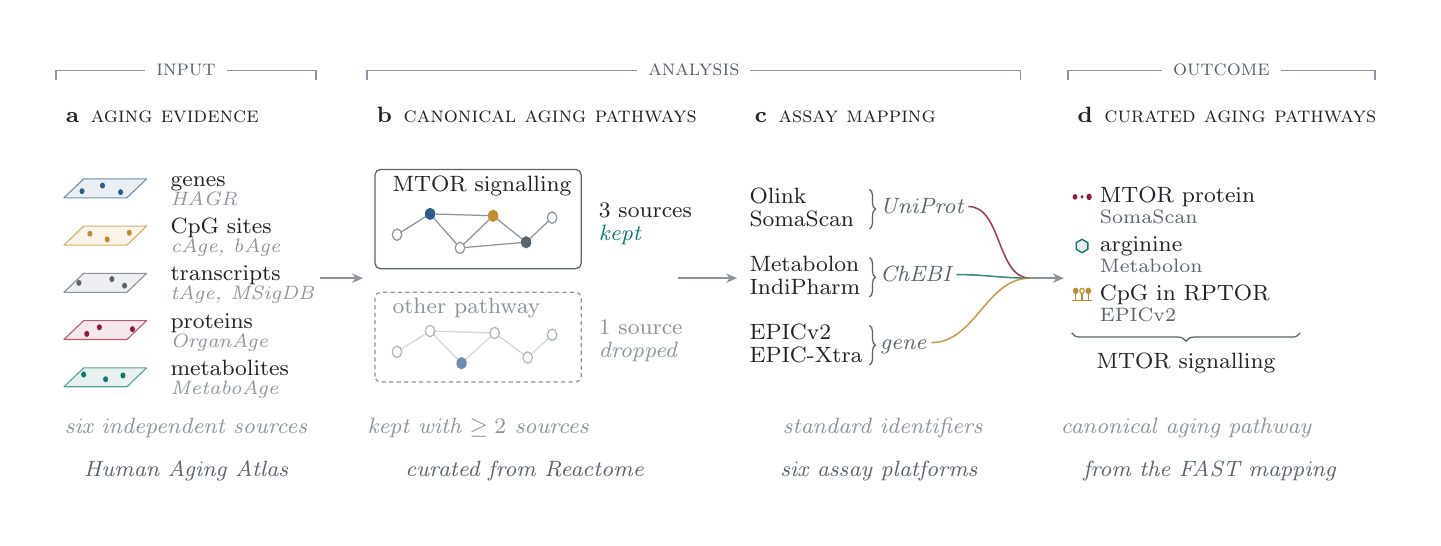
\begin{tikzpicture}[
    yscale=1.2,
    font=\footnotesize, text=ink,
    show background rectangle,
    background rectangle/.style={fill=white},
    inner frame sep=10pt,
    title/.style={anchor=base west, font=\footnotesize},
    sub/.style={anchor=base, text=mute, font=\footnotesize\itshape},
    tag/.style={anchor=north, text=faint, font=\footnotesize\itshape},
    flow/.style={draw=faint, line width=0.6pt, -{Stealth[length=4pt, width=3.4pt]}},
    group/.style={draw=faint, line width=0.5pt},
    grouplabel/.style={text=mute, font=\footnotesize\scshape, fill=white, inner xsep=4pt},
    link/.style={draw=ink!65, line width=0.45pt, -{Stealth[length=3pt, width=2.6pt]}},
    card/.style={draw=rule, line width=0.45pt, rounded corners=2pt}]

  % ---------------------------------------------------------- titles
  \node[title] at (-0.35,4.05) {\textbf{a}\enspace\textsc{aging evidence}};
  \node[title] at (3.60,4.05)  {\textbf{b}\enspace\textsc{canonical aging pathways}};
  \node[title] at (8.40,4.05)  {\textbf{c}\enspace\textsc{assay mapping}};
  \node[title] at (12.50,4.05) {\textbf{d}\enspace\textsc{curated aging pathways}};
  \draw[group] (-0.35,4.50) -- ++(0,0.10) -| (2.95,4.50);
  \node[grouplabel] at (1.30,4.60) {input};
  \draw[group] (3.60,4.50) -- ++(0,0.10) -| (11.90,4.50);
  \node[grouplabel] at (7.75,4.60) {analysis};
  \draw[group] (12.50,4.50) -- ++(0,0.10) -| (16.40,4.50);
  \node[grouplabel] at (14.45,4.60) {outcome};

  % ------------------------------------------------- a: aging evidence
  % one plane per omic layer of the Human Aging Atlas, with its published sources
  \layer{3.25}{slate}{-0.02/0.07, 0.24/0.13, 0.47/0.06}
  \layer{2.75}{ochre}{0.08/0.12, 0.30/0.06, 0.58/0.13}
  \layer{2.25}{mute}{-0.06/0.10, 0.36/0.14, 0.52/0.07}
  \layer{1.75}{risk}{0.04/0.06, 0.20/0.13, 0.62/0.11}
  \layer{1.25}{ml}{0.00/0.13, 0.28/0.08, 0.50/0.12}
  \foreach \y/\t/\s in {3.25/genes/HAGR, 2.75/CpG sites/{cAge, bAge}, 2.25/transcripts/{tAge, MSigDB},
      1.75/proteins/OrganAge, 1.25/metabolites/MetaboAge} {
    \node[anchor=base west] at (0.98,\y+0.12) {\t};
    \node[anchor=base west, text=faint, font=\scriptsize\itshape] at (0.98,\y-0.08) {\s};
  }
  \node[tag] at (1.30,1.02) {six independent sources};

  % ---------------------------------------- b: canonical aging pathways
  % a Reactome pathway is kept when two or more independent sources support its members
  \draw[card, draw=mute] (3.70,2.50) rectangle (6.32,3.55);
  \node[anchor=base west] at (3.80,3.32) {MTOR signalling};
  \draw[faint, line width=0.45pt] (3.98,2.86) -- (4.40,3.08) -- (4.78,2.72) -- (5.20,3.06) -- (5.62,2.78)
    -- (5.95,3.04) (4.40,3.08) -- (5.20,3.06) (4.78,2.72) -- (5.62,2.78);
  \foreach \x/\y in {3.98/2.86, 4.78/2.72, 5.95/3.04}
    \filldraw[fill=white, draw=faint, line width=0.45pt] (\x,\y) circle (0.06);
  \fill[slate] (4.40,3.08) circle (0.065);
  \fill[ochre] (5.20,3.06) circle (0.065);
  \fill[mute] (5.62,2.78) circle (0.065);
  \node[anchor=base west] at (6.42,3.04) {3 sources};
  \node[anchor=base west, text=ml, font=\footnotesize\itshape] at (6.42,2.80) {kept};

  \draw[card, draw=faint, dash pattern=on 1.5pt off 1.2pt] (3.70,1.30) rectangle (6.32,2.25);
  \node[anchor=base west, text=faint] at (3.80,2.03) {other pathway};
  \draw[rule, line width=0.45pt] (3.98,1.62) -- (4.40,1.84) -- (4.80,1.50) -- (5.22,1.82) -- (5.64,1.56)
    -- (5.95,1.80) (4.40,1.84) -- (5.22,1.82);
  \foreach \x/\y in {3.98/1.62, 4.40/1.84, 5.22/1.82, 5.64/1.56, 5.95/1.80}
    \filldraw[fill=white, draw=faint!70, line width=0.45pt] (\x,\y) circle (0.06);
  \fill[slate!70] (4.80,1.50) circle (0.065);
  \node[anchor=base west, text=faint] at (6.42,1.80) {1 source};
  \node[anchor=base west, text=faint, font=\footnotesize\itshape] at (6.42,1.56) {dropped};
  \node[tag] at (5.01,1.02) {kept with $\geq 2$ sources};

  % -------------------------------------------------- c: assay mapping
  % the two platforms of an omic layer share one identifier, which links their analytes to aging pathways
  \foreach \y/\a/\b/\i in {3.12/Olink/SomaScan/UniProt, 2.40/Metabolon/IndiPharm/ChEBI, 1.68/EPICv2/EPIC-Xtra/gene} {
    \node[anchor=base west, inner xsep=0pt] at (8.45,\y+0.07) {\a};
    \node[anchor=base west, inner xsep=0pt] at (8.45,\y-0.17) {\b};
    \draw[decorate, decoration={brace, amplitude=2.2pt}, mute, line width=0.45pt] (9.98,\y+0.22) -- (9.98,\y-0.20);
    \node[anchor=base west, inner xsep=0pt, text=mute, font=\footnotesize\itshape] (id-\i) at (10.11,\y-0.04) {\i};
  }
  % the identifiers lead into the analyte records, coloured by omic layer as in panel a
  \foreach \i/\c in {UniProt/risk, ChEBI/ml, gene/ochre}
    \draw[\c, line width=0.55pt, opacity=0.85] ([xshift=1.6pt, yshift=2.2pt]id-\i.base east) to[out=0, in=180] (12.02,2.40);
  \node[tag] at (10.15,1.02) {standard identifiers};

  % ------------------------------------------ d: curated aging pathways
  % assays on three platforms that belong to one canonical aging pathway, taken from the FAST mapping
  \foreach \y/\g/\a/\p in {3.20/protein/MTOR protein/SomaScan, 2.68/metabolite/arginine/Metabolon, 2.16/cpg/CpG in RPTOR/EPICv2} {
    \begin{scope}[shift={(12.68,\y+0.06)}] \csname\g\endcsname \end{scope}
    \node[anchor=base west, inner xsep=0pt] at (12.90,\y) {\a};
    \node[anchor=base west, inner xsep=0pt, text=mute, font=\scriptsize] at (12.90,\y-0.22) {\p};
  }
  \draw[decorate, decoration={brace, amplitude=3pt}, mute, line width=0.45pt] (15.45,1.82) -- (12.55,1.82);
  \node[anchor=base] at (14.00,1.44) {MTOR signalling};
  \node[tag] at (14.00,1.02) {canonical aging pathway};

  % --------------------------------------------------- panel notes
  \node[sub] at (1.30,0.30)  {Human Aging Atlas};
  \node[sub] at (5.60,0.30)  {curated from Reactome};
  \node[sub] at (10.10,0.30) {six assay platforms};
  \node[sub] at (14.30,0.30) {from the FAST mapping};

  \draw[flow] (3.00,2.40) -- (3.55,2.40);
  \draw[flow] (7.55,2.40) -- (8.30,2.40);
  \draw[flow] (12.02,2.40) -- (12.45,2.40);
\end{tikzpicture}
\end{document}
"
%          dvisvgm --no-fonts --exact-bbox --optimize research_fast.dvi
\documentclass[tikz,border=0pt]{standalone}
\usepackage[T1]{fontenc}
\usepackage{lmodern}
\usepackage{amsmath}
\usetikzlibrary{arrows.meta,backgrounds,decorations.pathreplacing}

\definecolor{ink}{HTML}{1F2328}
\definecolor{mute}{HTML}{59636E}
\definecolor{faint}{HTML}{8C959F}
\definecolor{rule}{HTML}{D0D7DE}
\definecolor{risk}{HTML}{8E1B3A}
\definecolor{ochre}{HTML}{C08A2E}
\definecolor{slate}{HTML}{2F5C8A}
\definecolor{ml}{HTML}{0F766E}

% omic layer of panel a: #1 bottom edge, #2 colour, #3 entities as x/height pairs
\newcommand{\layer}[3]{%
  \filldraw[fill=#2!10, draw=#2!70, line width=0.4pt, line join=round]
    (-0.25,#1) -- (0.55,#1) -- (0.80,#1+0.20) -- (0.00,#1+0.20) -- cycle;
  \foreach \u/\v in {#3} \fill[#2] (\u,#1+\v) circle (0.032);}
% analyte glyphs of panel d, with the colour of the omic layer in panel a
\newcommand{\protein}[1][risk]{%
  \foreach \i/\r in {0/0.030, 1/0.020, 2/0.034} \fill[#1] (-0.09+0.09*\i,0) circle (\r);}
\newcommand{\metabolite}{%
  \filldraw[fill=ml!12, draw=ml, line width=0.5pt, line join=round, yscale=0.833]
    (90:0.085) -- (150:0.085) -- (210:0.085) -- (270:0.085) -- (330:0.085) -- (30:0.085) -- cycle;}
\newcommand{\cpg}{%
  \draw[ochre, line width=0.45pt] (-0.13,-0.06) -- (0.13,-0.06);
  \foreach \x/\f in {-0.08/ochre, 0.00/white, 0.08/ochre} {
    \draw[ochre, line width=0.45pt] (\x,-0.06) -- (\x,0.02);
    \filldraw[fill=\f, draw=ochre, line width=0.4pt] (\x,0.045) circle (0.028);
  }}

\begin{document}
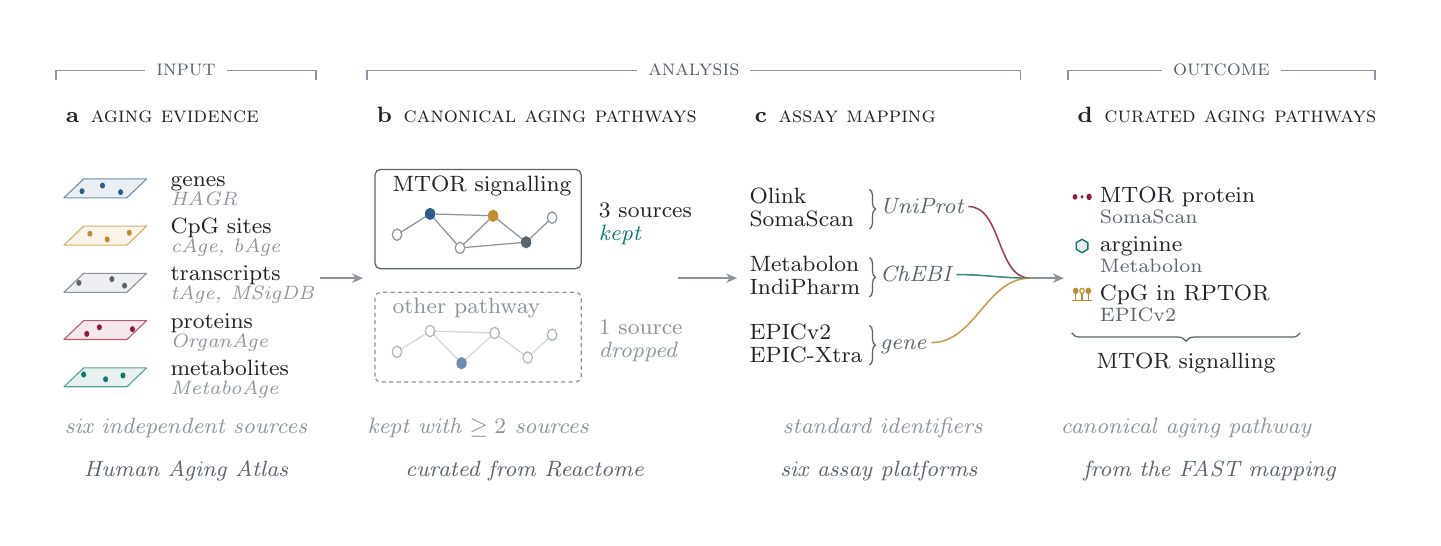
\begin{tikzpicture}[
    yscale=1.2,
    font=\footnotesize, text=ink,
    show background rectangle,
    background rectangle/.style={fill=white},
    inner frame sep=10pt,
    title/.style={anchor=base west, font=\footnotesize},
    sub/.style={anchor=base, text=mute, font=\footnotesize\itshape},
    tag/.style={anchor=north, text=faint, font=\footnotesize\itshape},
    flow/.style={draw=faint, line width=0.6pt, -{Stealth[length=4pt, width=3.4pt]}},
    group/.style={draw=faint, line width=0.5pt},
    grouplabel/.style={text=mute, font=\footnotesize\scshape, fill=white, inner xsep=4pt},
    link/.style={draw=ink!65, line width=0.45pt, -{Stealth[length=3pt, width=2.6pt]}},
    card/.style={draw=rule, line width=0.45pt, rounded corners=2pt}]

  % ---------------------------------------------------------- titles
  \node[title] at (-0.35,4.05) {\textbf{a}\enspace\textsc{aging evidence}};
  \node[title] at (3.60,4.05)  {\textbf{b}\enspace\textsc{canonical aging pathways}};
  \node[title] at (8.40,4.05)  {\textbf{c}\enspace\textsc{assay mapping}};
  \node[title] at (12.50,4.05) {\textbf{d}\enspace\textsc{curated aging pathways}};
  \draw[group] (-0.35,4.50) -- ++(0,0.10) -| (2.95,4.50);
  \node[grouplabel] at (1.30,4.60) {input};
  \draw[group] (3.60,4.50) -- ++(0,0.10) -| (11.90,4.50);
  \node[grouplabel] at (7.75,4.60) {analysis};
  \draw[group] (12.50,4.50) -- ++(0,0.10) -| (16.40,4.50);
  \node[grouplabel] at (14.45,4.60) {outcome};

  % ------------------------------------------------- a: aging evidence
  % one plane per omic layer of the Human Aging Atlas, with its published sources
  \layer{3.25}{slate}{-0.02/0.07, 0.24/0.13, 0.47/0.06}
  \layer{2.75}{ochre}{0.08/0.12, 0.30/0.06, 0.58/0.13}
  \layer{2.25}{mute}{-0.06/0.10, 0.36/0.14, 0.52/0.07}
  \layer{1.75}{risk}{0.04/0.06, 0.20/0.13, 0.62/0.11}
  \layer{1.25}{ml}{0.00/0.13, 0.28/0.08, 0.50/0.12}
  \foreach \y/\t/\s in {3.25/genes/HAGR, 2.75/CpG sites/{cAge, bAge}, 2.25/transcripts/{tAge, MSigDB},
      1.75/proteins/OrganAge, 1.25/metabolites/MetaboAge} {
    \node[anchor=base west] at (0.98,\y+0.12) {\t};
    \node[anchor=base west, text=faint, font=\scriptsize\itshape] at (0.98,\y-0.08) {\s};
  }
  \node[tag] at (1.30,1.02) {six independent sources};

  % ---------------------------------------- b: canonical aging pathways
  % a Reactome pathway is kept when two or more independent sources support its members
  \draw[card, draw=mute] (3.70,2.50) rectangle (6.32,3.55);
  \node[anchor=base west] at (3.80,3.32) {MTOR signalling};
  \draw[faint, line width=0.45pt] (3.98,2.86) -- (4.40,3.08) -- (4.78,2.72) -- (5.20,3.06) -- (5.62,2.78)
    -- (5.95,3.04) (4.40,3.08) -- (5.20,3.06) (4.78,2.72) -- (5.62,2.78);
  \foreach \x/\y in {3.98/2.86, 4.78/2.72, 5.95/3.04}
    \filldraw[fill=white, draw=faint, line width=0.45pt] (\x,\y) circle (0.06);
  \fill[slate] (4.40,3.08) circle (0.065);
  \fill[ochre] (5.20,3.06) circle (0.065);
  \fill[mute] (5.62,2.78) circle (0.065);
  \node[anchor=base west] at (6.42,3.04) {3 sources};
  \node[anchor=base west, text=ml, font=\footnotesize\itshape] at (6.42,2.80) {kept};

  \draw[card, draw=faint, dash pattern=on 1.5pt off 1.2pt] (3.70,1.30) rectangle (6.32,2.25);
  \node[anchor=base west, text=faint] at (3.80,2.03) {other pathway};
  \draw[rule, line width=0.45pt] (3.98,1.62) -- (4.40,1.84) -- (4.80,1.50) -- (5.22,1.82) -- (5.64,1.56)
    -- (5.95,1.80) (4.40,1.84) -- (5.22,1.82);
  \foreach \x/\y in {3.98/1.62, 4.40/1.84, 5.22/1.82, 5.64/1.56, 5.95/1.80}
    \filldraw[fill=white, draw=faint!70, line width=0.45pt] (\x,\y) circle (0.06);
  \fill[slate!70] (4.80,1.50) circle (0.065);
  \node[anchor=base west, text=faint] at (6.42,1.80) {1 source};
  \node[anchor=base west, text=faint, font=\footnotesize\itshape] at (6.42,1.56) {dropped};
  \node[tag] at (5.01,1.02) {kept with $\geq 2$ sources};

  % -------------------------------------------------- c: assay mapping
  % the two platforms of an omic layer share one identifier, which links their analytes to aging pathways
  \foreach \y/\a/\b/\i in {3.12/Olink/SomaScan/UniProt, 2.40/Metabolon/IndiPharm/ChEBI, 1.68/EPICv2/EPIC-Xtra/gene} {
    \node[anchor=base west, inner xsep=0pt] at (8.45,\y+0.07) {\a};
    \node[anchor=base west, inner xsep=0pt] at (8.45,\y-0.17) {\b};
    \draw[decorate, decoration={brace, amplitude=2.2pt}, mute, line width=0.45pt] (9.98,\y+0.22) -- (9.98,\y-0.20);
    \node[anchor=base west, inner xsep=0pt, text=mute, font=\footnotesize\itshape] (id-\i) at (10.11,\y-0.04) {\i};
  }
  % the identifiers lead into the analyte records, coloured by omic layer as in panel a
  \foreach \i/\c in {UniProt/risk, ChEBI/ml, gene/ochre}
    \draw[\c, line width=0.55pt, opacity=0.85] ([xshift=1.6pt, yshift=2.2pt]id-\i.base east) to[out=0, in=180] (12.02,2.40);
  \node[tag] at (10.15,1.02) {standard identifiers};

  % ------------------------------------------ d: curated aging pathways
  % assays on three platforms that belong to one canonical aging pathway, taken from the FAST mapping
  \foreach \y/\g/\a/\p in {3.20/protein/MTOR protein/SomaScan, 2.68/metabolite/arginine/Metabolon, 2.16/cpg/CpG in RPTOR/EPICv2} {
    \begin{scope}[shift={(12.68,\y+0.06)}] \csname\g\endcsname \end{scope}
    \node[anchor=base west, inner xsep=0pt] at (12.90,\y) {\a};
    \node[anchor=base west, inner xsep=0pt, text=mute, font=\scriptsize] at (12.90,\y-0.22) {\p};
  }
  \draw[decorate, decoration={brace, amplitude=3pt}, mute, line width=0.45pt] (15.45,1.82) -- (12.55,1.82);
  \node[anchor=base] at (14.00,1.44) {MTOR signalling};
  \node[tag] at (14.00,1.02) {canonical aging pathway};

  % --------------------------------------------------- panel notes
  \node[sub] at (1.30,0.30)  {Human Aging Atlas};
  \node[sub] at (5.60,0.30)  {curated from Reactome};
  \node[sub] at (10.10,0.30) {six assay platforms};
  \node[sub] at (14.30,0.30) {from the FAST mapping};

  \draw[flow] (3.00,2.40) -- (3.55,2.40);
  \draw[flow] (7.55,2.40) -- (8.30,2.40);
  \draw[flow] (12.02,2.40) -- (12.45,2.40);
\end{tikzpicture}
\end{document}
"
%          dvisvgm --no-fonts --exact-bbox --optimize research_fast.dvi
\documentclass[tikz,border=0pt]{standalone}
\usepackage[T1]{fontenc}
\usepackage{lmodern}
\usepackage{amsmath}
\usetikzlibrary{arrows.meta,backgrounds,decorations.pathreplacing}

\definecolor{ink}{HTML}{1F2328}
\definecolor{mute}{HTML}{59636E}
\definecolor{faint}{HTML}{8C959F}
\definecolor{rule}{HTML}{D0D7DE}
\definecolor{risk}{HTML}{8E1B3A}
\definecolor{ochre}{HTML}{C08A2E}
\definecolor{slate}{HTML}{2F5C8A}
\definecolor{ml}{HTML}{0F766E}

% omic layer of panel a: #1 bottom edge, #2 colour, #3 entities as x/height pairs
\newcommand{\layer}[3]{%
  \filldraw[fill=#2!10, draw=#2!70, line width=0.4pt, line join=round]
    (-0.25,#1) -- (0.55,#1) -- (0.80,#1+0.20) -- (0.00,#1+0.20) -- cycle;
  \foreach \u/\v in {#3} \fill[#2] (\u,#1+\v) circle (0.032);}
% analyte glyphs of panel d, with the colour of the omic layer in panel a
\newcommand{\protein}[1][risk]{%
  \foreach \i/\r in {0/0.030, 1/0.020, 2/0.034} \fill[#1] (-0.09+0.09*\i,0) circle (\r);}
\newcommand{\metabolite}{%
  \filldraw[fill=ml!12, draw=ml, line width=0.5pt, line join=round, yscale=0.833]
    (90:0.085) -- (150:0.085) -- (210:0.085) -- (270:0.085) -- (330:0.085) -- (30:0.085) -- cycle;}
\newcommand{\cpg}{%
  \draw[ochre, line width=0.45pt] (-0.13,-0.06) -- (0.13,-0.06);
  \foreach \x/\f in {-0.08/ochre, 0.00/white, 0.08/ochre} {
    \draw[ochre, line width=0.45pt] (\x,-0.06) -- (\x,0.02);
    \filldraw[fill=\f, draw=ochre, line width=0.4pt] (\x,0.045) circle (0.028);
  }}

\begin{document}
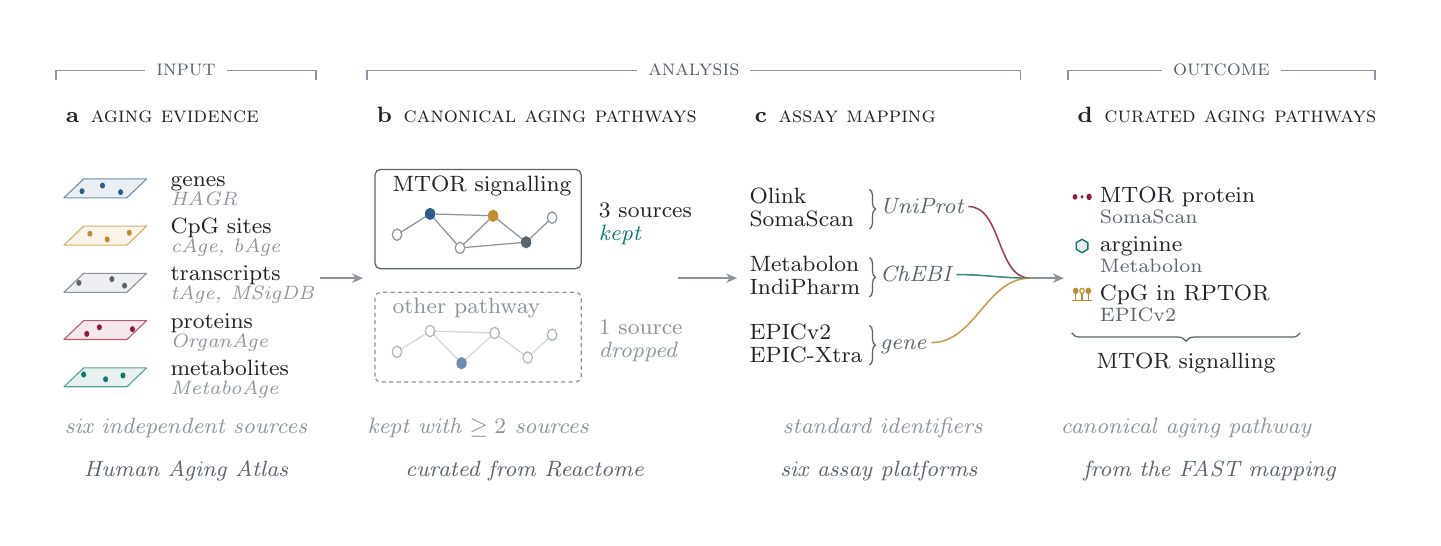
\begin{tikzpicture}[
    yscale=1.2,
    font=\footnotesize, text=ink,
    show background rectangle,
    background rectangle/.style={fill=white},
    inner frame sep=10pt,
    title/.style={anchor=base west, font=\footnotesize},
    sub/.style={anchor=base, text=mute, font=\footnotesize\itshape},
    tag/.style={anchor=north, text=faint, font=\footnotesize\itshape},
    flow/.style={draw=faint, line width=0.6pt, -{Stealth[length=4pt, width=3.4pt]}},
    group/.style={draw=faint, line width=0.5pt},
    grouplabel/.style={text=mute, font=\footnotesize\scshape, fill=white, inner xsep=4pt},
    link/.style={draw=ink!65, line width=0.45pt, -{Stealth[length=3pt, width=2.6pt]}},
    card/.style={draw=rule, line width=0.45pt, rounded corners=2pt}]

  % ---------------------------------------------------------- titles
  \node[title] at (-0.35,4.05) {\textbf{a}\enspace\textsc{aging evidence}};
  \node[title] at (3.60,4.05)  {\textbf{b}\enspace\textsc{canonical aging pathways}};
  \node[title] at (8.40,4.05)  {\textbf{c}\enspace\textsc{assay mapping}};
  \node[title] at (12.50,4.05) {\textbf{d}\enspace\textsc{curated aging pathways}};
  \draw[group] (-0.35,4.50) -- ++(0,0.10) -| (2.95,4.50);
  \node[grouplabel] at (1.30,4.60) {input};
  \draw[group] (3.60,4.50) -- ++(0,0.10) -| (11.90,4.50);
  \node[grouplabel] at (7.75,4.60) {analysis};
  \draw[group] (12.50,4.50) -- ++(0,0.10) -| (16.40,4.50);
  \node[grouplabel] at (14.45,4.60) {outcome};

  % ------------------------------------------------- a: aging evidence
  % one plane per omic layer of the Human Aging Atlas, with its published sources
  \layer{3.25}{slate}{-0.02/0.07, 0.24/0.13, 0.47/0.06}
  \layer{2.75}{ochre}{0.08/0.12, 0.30/0.06, 0.58/0.13}
  \layer{2.25}{mute}{-0.06/0.10, 0.36/0.14, 0.52/0.07}
  \layer{1.75}{risk}{0.04/0.06, 0.20/0.13, 0.62/0.11}
  \layer{1.25}{ml}{0.00/0.13, 0.28/0.08, 0.50/0.12}
  \foreach \y/\t/\s in {3.25/genes/HAGR, 2.75/CpG sites/{cAge, bAge}, 2.25/transcripts/{tAge, MSigDB},
      1.75/proteins/OrganAge, 1.25/metabolites/MetaboAge} {
    \node[anchor=base west] at (0.98,\y+0.12) {\t};
    \node[anchor=base west, text=faint, font=\scriptsize\itshape] at (0.98,\y-0.08) {\s};
  }
  \node[tag] at (1.30,1.02) {six independent sources};

  % ---------------------------------------- b: canonical aging pathways
  % a Reactome pathway is kept when two or more independent sources support its members
  \draw[card, draw=mute] (3.70,2.50) rectangle (6.32,3.55);
  \node[anchor=base west] at (3.80,3.32) {MTOR signalling};
  \draw[faint, line width=0.45pt] (3.98,2.86) -- (4.40,3.08) -- (4.78,2.72) -- (5.20,3.06) -- (5.62,2.78)
    -- (5.95,3.04) (4.40,3.08) -- (5.20,3.06) (4.78,2.72) -- (5.62,2.78);
  \foreach \x/\y in {3.98/2.86, 4.78/2.72, 5.95/3.04}
    \filldraw[fill=white, draw=faint, line width=0.45pt] (\x,\y) circle (0.06);
  \fill[slate] (4.40,3.08) circle (0.065);
  \fill[ochre] (5.20,3.06) circle (0.065);
  \fill[mute] (5.62,2.78) circle (0.065);
  \node[anchor=base west] at (6.42,3.04) {3 sources};
  \node[anchor=base west, text=ml, font=\footnotesize\itshape] at (6.42,2.80) {kept};

  \draw[card, draw=faint, dash pattern=on 1.5pt off 1.2pt] (3.70,1.30) rectangle (6.32,2.25);
  \node[anchor=base west, text=faint] at (3.80,2.03) {other pathway};
  \draw[rule, line width=0.45pt] (3.98,1.62) -- (4.40,1.84) -- (4.80,1.50) -- (5.22,1.82) -- (5.64,1.56)
    -- (5.95,1.80) (4.40,1.84) -- (5.22,1.82);
  \foreach \x/\y in {3.98/1.62, 4.40/1.84, 5.22/1.82, 5.64/1.56, 5.95/1.80}
    \filldraw[fill=white, draw=faint!70, line width=0.45pt] (\x,\y) circle (0.06);
  \fill[slate!70] (4.80,1.50) circle (0.065);
  \node[anchor=base west, text=faint] at (6.42,1.80) {1 source};
  \node[anchor=base west, text=faint, font=\footnotesize\itshape] at (6.42,1.56) {dropped};
  \node[tag] at (5.01,1.02) {kept with $\geq 2$ sources};

  % -------------------------------------------------- c: assay mapping
  % the two platforms of an omic layer share one identifier, which links their analytes to aging pathways
  \foreach \y/\a/\b/\i in {3.12/Olink/SomaScan/UniProt, 2.40/Metabolon/IndiPharm/ChEBI, 1.68/EPICv2/EPIC-Xtra/gene} {
    \node[anchor=base west, inner xsep=0pt] at (8.45,\y+0.07) {\a};
    \node[anchor=base west, inner xsep=0pt] at (8.45,\y-0.17) {\b};
    \draw[decorate, decoration={brace, amplitude=2.2pt}, mute, line width=0.45pt] (9.98,\y+0.22) -- (9.98,\y-0.20);
    \node[anchor=base west, inner xsep=0pt, text=mute, font=\footnotesize\itshape] (id-\i) at (10.11,\y-0.04) {\i};
  }
  % the identifiers lead into the analyte records, coloured by omic layer as in panel a
  \foreach \i/\c in {UniProt/risk, ChEBI/ml, gene/ochre}
    \draw[\c, line width=0.55pt, opacity=0.85] ([xshift=1.6pt, yshift=2.2pt]id-\i.base east) to[out=0, in=180] (12.02,2.40);
  \node[tag] at (10.15,1.02) {standard identifiers};

  % ------------------------------------------ d: curated aging pathways
  % assays on three platforms that belong to one canonical aging pathway, taken from the FAST mapping
  \foreach \y/\g/\a/\p in {3.20/protein/MTOR protein/SomaScan, 2.68/metabolite/arginine/Metabolon, 2.16/cpg/CpG in RPTOR/EPICv2} {
    \begin{scope}[shift={(12.68,\y+0.06)}] \csname\g\endcsname \end{scope}
    \node[anchor=base west, inner xsep=0pt] at (12.90,\y) {\a};
    \node[anchor=base west, inner xsep=0pt, text=mute, font=\scriptsize] at (12.90,\y-0.22) {\p};
  }
  \draw[decorate, decoration={brace, amplitude=3pt}, mute, line width=0.45pt] (15.45,1.82) -- (12.55,1.82);
  \node[anchor=base] at (14.00,1.44) {MTOR signalling};
  \node[tag] at (14.00,1.02) {canonical aging pathway};

  % --------------------------------------------------- panel notes
  \node[sub] at (1.30,0.30)  {Human Aging Atlas};
  \node[sub] at (5.60,0.30)  {curated from Reactome};
  \node[sub] at (10.10,0.30) {six assay platforms};
  \node[sub] at (14.30,0.30) {from the FAST mapping};

  \draw[flow] (3.00,2.40) -- (3.55,2.40);
  \draw[flow] (7.55,2.40) -- (8.30,2.40);
  \draw[flow] (12.02,2.40) -- (12.45,2.40);
\end{tikzpicture}
\end{document}
"
%          dvisvgm --no-fonts --exact-bbox --optimize research_fast.dvi
\documentclass[tikz,border=0pt]{standalone}
\usepackage[T1]{fontenc}
\usepackage{lmodern}
\usepackage{amsmath}
\usetikzlibrary{arrows.meta,backgrounds,decorations.pathreplacing}

\definecolor{ink}{HTML}{1F2328}
\definecolor{mute}{HTML}{59636E}
\definecolor{faint}{HTML}{8C959F}
\definecolor{rule}{HTML}{D0D7DE}
\definecolor{risk}{HTML}{8E1B3A}
\definecolor{ochre}{HTML}{C08A2E}
\definecolor{slate}{HTML}{2F5C8A}
\definecolor{ml}{HTML}{0F766E}

% omic layer of panel a: #1 bottom edge, #2 colour, #3 entities as x/height pairs
\newcommand{\layer}[3]{%
  \filldraw[fill=#2!10, draw=#2!70, line width=0.4pt, line join=round]
    (-0.25,#1) -- (0.55,#1) -- (0.80,#1+0.20) -- (0.00,#1+0.20) -- cycle;
  \foreach \u/\v in {#3} \fill[#2] (\u,#1+\v) circle (0.032);}
% analyte glyphs of panel d, with the colour of the omic layer in panel a
\newcommand{\protein}[1][risk]{%
  \foreach \i/\r in {0/0.030, 1/0.020, 2/0.034} \fill[#1] (-0.09+0.09*\i,0) circle (\r);}
\newcommand{\metabolite}{%
  \filldraw[fill=ml!12, draw=ml, line width=0.5pt, line join=round, yscale=0.833]
    (90:0.085) -- (150:0.085) -- (210:0.085) -- (270:0.085) -- (330:0.085) -- (30:0.085) -- cycle;}
\newcommand{\cpg}{%
  \draw[ochre, line width=0.45pt] (-0.13,-0.06) -- (0.13,-0.06);
  \foreach \x/\f in {-0.08/ochre, 0.00/white, 0.08/ochre} {
    \draw[ochre, line width=0.45pt] (\x,-0.06) -- (\x,0.02);
    \filldraw[fill=\f, draw=ochre, line width=0.4pt] (\x,0.045) circle (0.028);
  }}

\begin{document}
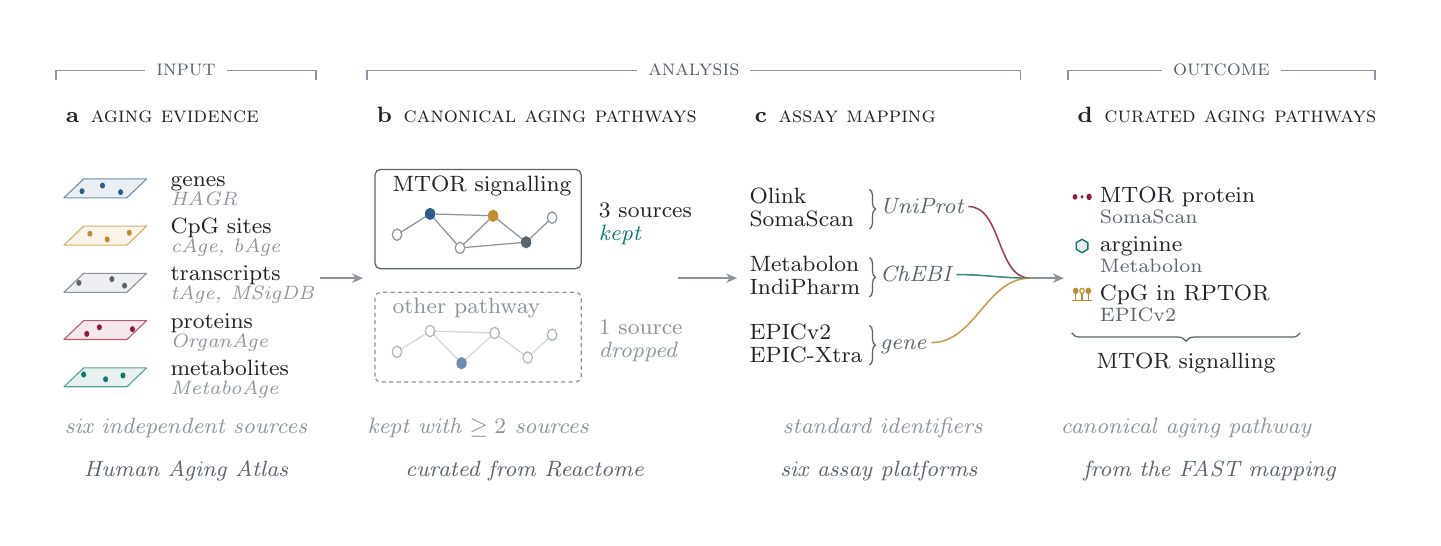
\begin{tikzpicture}[
    yscale=1.2,
    font=\footnotesize, text=ink,
    show background rectangle,
    background rectangle/.style={fill=white},
    inner frame sep=10pt,
    title/.style={anchor=base west, font=\footnotesize},
    sub/.style={anchor=base, text=mute, font=\footnotesize\itshape},
    tag/.style={anchor=north, text=faint, font=\footnotesize\itshape},
    flow/.style={draw=faint, line width=0.6pt, -{Stealth[length=4pt, width=3.4pt]}},
    group/.style={draw=faint, line width=0.5pt},
    grouplabel/.style={text=mute, font=\footnotesize\scshape, fill=white, inner xsep=4pt},
    link/.style={draw=ink!65, line width=0.45pt, -{Stealth[length=3pt, width=2.6pt]}},
    card/.style={draw=rule, line width=0.45pt, rounded corners=2pt}]

  % ---------------------------------------------------------- titles
  \node[title] at (-0.35,4.05) {\textbf{a}\enspace\textsc{aging evidence}};
  \node[title] at (3.60,4.05)  {\textbf{b}\enspace\textsc{canonical aging pathways}};
  \node[title] at (8.40,4.05)  {\textbf{c}\enspace\textsc{assay mapping}};
  \node[title] at (12.50,4.05) {\textbf{d}\enspace\textsc{curated aging pathways}};
  \draw[group] (-0.35,4.50) -- ++(0,0.10) -| (2.95,4.50);
  \node[grouplabel] at (1.30,4.60) {input};
  \draw[group] (3.60,4.50) -- ++(0,0.10) -| (11.90,4.50);
  \node[grouplabel] at (7.75,4.60) {analysis};
  \draw[group] (12.50,4.50) -- ++(0,0.10) -| (16.40,4.50);
  \node[grouplabel] at (14.45,4.60) {outcome};

  % ------------------------------------------------- a: aging evidence
  % one plane per omic layer of the Human Aging Atlas, with its published sources
  \layer{3.25}{slate}{-0.02/0.07, 0.24/0.13, 0.47/0.06}
  \layer{2.75}{ochre}{0.08/0.12, 0.30/0.06, 0.58/0.13}
  \layer{2.25}{mute}{-0.06/0.10, 0.36/0.14, 0.52/0.07}
  \layer{1.75}{risk}{0.04/0.06, 0.20/0.13, 0.62/0.11}
  \layer{1.25}{ml}{0.00/0.13, 0.28/0.08, 0.50/0.12}
  \foreach \y/\t/\s in {3.25/genes/HAGR, 2.75/CpG sites/{cAge, bAge}, 2.25/transcripts/{tAge, MSigDB},
      1.75/proteins/OrganAge, 1.25/metabolites/MetaboAge} {
    \node[anchor=base west] at (0.98,\y+0.12) {\t};
    \node[anchor=base west, text=faint, font=\scriptsize\itshape] at (0.98,\y-0.08) {\s};
  }
  \node[tag] at (1.30,1.02) {six independent sources};

  % ---------------------------------------- b: canonical aging pathways
  % a Reactome pathway is kept when two or more independent sources support its members
  \draw[card, draw=mute] (3.70,2.50) rectangle (6.32,3.55);
  \node[anchor=base west] at (3.80,3.32) {MTOR signalling};
  \draw[faint, line width=0.45pt] (3.98,2.86) -- (4.40,3.08) -- (4.78,2.72) -- (5.20,3.06) -- (5.62,2.78)
    -- (5.95,3.04) (4.40,3.08) -- (5.20,3.06) (4.78,2.72) -- (5.62,2.78);
  \foreach \x/\y in {3.98/2.86, 4.78/2.72, 5.95/3.04}
    \filldraw[fill=white, draw=faint, line width=0.45pt] (\x,\y) circle (0.06);
  \fill[slate] (4.40,3.08) circle (0.065);
  \fill[ochre] (5.20,3.06) circle (0.065);
  \fill[mute] (5.62,2.78) circle (0.065);
  \node[anchor=base west] at (6.42,3.04) {3 sources};
  \node[anchor=base west, text=ml, font=\footnotesize\itshape] at (6.42,2.80) {kept};

  \draw[card, draw=faint, dash pattern=on 1.5pt off 1.2pt] (3.70,1.30) rectangle (6.32,2.25);
  \node[anchor=base west, text=faint] at (3.80,2.03) {other pathway};
  \draw[rule, line width=0.45pt] (3.98,1.62) -- (4.40,1.84) -- (4.80,1.50) -- (5.22,1.82) -- (5.64,1.56)
    -- (5.95,1.80) (4.40,1.84) -- (5.22,1.82);
  \foreach \x/\y in {3.98/1.62, 4.40/1.84, 5.22/1.82, 5.64/1.56, 5.95/1.80}
    \filldraw[fill=white, draw=faint!70, line width=0.45pt] (\x,\y) circle (0.06);
  \fill[slate!70] (4.80,1.50) circle (0.065);
  \node[anchor=base west, text=faint] at (6.42,1.80) {1 source};
  \node[anchor=base west, text=faint, font=\footnotesize\itshape] at (6.42,1.56) {dropped};
  \node[tag] at (5.01,1.02) {kept with $\geq 2$ sources};

  % -------------------------------------------------- c: assay mapping
  % the two platforms of an omic layer share one identifier, which links their analytes to aging pathways
  \foreach \y/\a/\b/\i in {3.12/Olink/SomaScan/UniProt, 2.40/Metabolon/IndiPharm/ChEBI, 1.68/EPICv2/EPIC-Xtra/gene} {
    \node[anchor=base west, inner xsep=0pt] at (8.45,\y+0.07) {\a};
    \node[anchor=base west, inner xsep=0pt] at (8.45,\y-0.17) {\b};
    \draw[decorate, decoration={brace, amplitude=2.2pt}, mute, line width=0.45pt] (9.98,\y+0.22) -- (9.98,\y-0.20);
    \node[anchor=base west, inner xsep=0pt, text=mute, font=\footnotesize\itshape] (id-\i) at (10.11,\y-0.04) {\i};
  }
  % the identifiers lead into the analyte records, coloured by omic layer as in panel a
  \foreach \i/\c in {UniProt/risk, ChEBI/ml, gene/ochre}
    \draw[\c, line width=0.55pt, opacity=0.85] ([xshift=1.6pt, yshift=2.2pt]id-\i.base east) to[out=0, in=180] (12.02,2.40);
  \node[tag] at (10.15,1.02) {standard identifiers};

  % ------------------------------------------ d: curated aging pathways
  % assays on three platforms that belong to one canonical aging pathway, taken from the FAST mapping
  \foreach \y/\g/\a/\p in {3.20/protein/MTOR protein/SomaScan, 2.68/metabolite/arginine/Metabolon, 2.16/cpg/CpG in RPTOR/EPICv2} {
    \begin{scope}[shift={(12.68,\y+0.06)}] \csname\g\endcsname \end{scope}
    \node[anchor=base west, inner xsep=0pt] at (12.90,\y) {\a};
    \node[anchor=base west, inner xsep=0pt, text=mute, font=\scriptsize] at (12.90,\y-0.22) {\p};
  }
  \draw[decorate, decoration={brace, amplitude=3pt}, mute, line width=0.45pt] (15.45,1.82) -- (12.55,1.82);
  \node[anchor=base] at (14.00,1.44) {MTOR signalling};
  \node[tag] at (14.00,1.02) {canonical aging pathway};

  % --------------------------------------------------- panel notes
  \node[sub] at (1.30,0.30)  {Human Aging Atlas};
  \node[sub] at (5.60,0.30)  {curated from Reactome};
  \node[sub] at (10.10,0.30) {six assay platforms};
  \node[sub] at (14.30,0.30) {from the FAST mapping};

  \draw[flow] (3.00,2.40) -- (3.55,2.40);
  \draw[flow] (7.55,2.40) -- (8.30,2.40);
  \draw[flow] (12.02,2.40) -- (12.45,2.40);
\end{tikzpicture}
\end{document}
